\documentclass[11pt]{article}
\usepackage[a4paper, total={6.8in, 9.25in}]{geometry}
\usepackage{graphicx}
\graphicspath{ {./assets/images/output/} }
\usepackage{caption}
\usepackage[english]{babel}
\usepackage{titling}
\usepackage{float}
\usepackage{amsmath}
\usepackage{algorithm}
\usepackage{algorithmicx}
\usepackage{algpseudocode}
\usepackage{minted}
\usepackage{multicol}
\usepackage{array}
\usepackage{setspace}
\usepackage{placeins}
\usepackage{tcolorbox}
\usepackage{caption}
\usepackage{subcaption}

\definecolor{verbgray}{gray}{.95}
\setminted{
    bgcolor=verbgray,
    baselinestretch=1,
    fontsize=\footnotesize,
    linenos,
    breaklines=true,
    breakanywhere=true,
    xleftmargin=\parindent
}
\title{Implementation of Linear and Logistic Regression for Regression and Classification Problems}
\author{}
\date{}

\pagenumbering{gobble}
\begin{document}
\input{ml_cover.tex}

\pagebreak

\tableofcontents

\pagebreak
\pagenumbering{arabic}
\maketitle

\section{Theory and Introduction}
The K-Nearest Neighbors (KNN) algorithm is a non-parametric, lazy learning algorithm used for both classification and regression. Unlike eager learning methods (e.g., Logistic Regression), KNN does not build a model during the training phase. Instead, it stores the entire training dataset and performs computation only during the prediction phase \cite{bishop2006pattern}.

\subsection{Classification Mechanism}
Given a new data point $x_{query}$, the algorithm identifies the $k$ training samples closest to it. The class label is determined by a majority vote among its $k$ nearest neighbors:
\begin{equation}
    \hat{y} = \text{mode}(\{ y_i : (x_i, y_i) \in N_k(x_{query}) \})
\end{equation}
where $N_k(x_{query})$ is the set of $k$ nearest neighbors.

\subsection{Distance Metrics}
The "closeness" between points is defined by a distance metric. Two common metrics were implemented in this study:

\subsubsection*{Euclidean Distance}
The straight-line distance between two points $p$ and $q$ in an $n$-dimensional space:
\begin{equation}
    d_{Euclidean}(p, q) = \sqrt{\sum_{i=1}^{n} (p_i - q_i)^2}
\end{equation}

\subsubsection*{Manhattan Distance}
The sum of absolute differences between the coordinates of the points (also known as $L_1$ norm):
\begin{equation}
    d_{Manhattan}(p, q) = \sum_{i=1}^{n} |p_i - q_i|
\end{equation}

\section{Methodology}

\subsection{Dataset}
The \textit{Iris} dataset was used, consisting of 150 samples across three classes: \textit{Setosa}, \textit{Versicolor}, and \textit{Virginica}. For visualization purposes, two features (Petal Length and Petal Width) were selected. The data was split into training (80\%) and testing (20\%) sets \cite{fisher1936use}.

\subsection{Algorithm Implementation}
The algorithm was implemented using Python (NumPy) without relying on high-level libraries like Scikit-Learn.

\begin{algorithm}[H]
    \caption{K-Nearest Neighbors (Prediction Phase)}
    \begin{algorithmic}[1]
        \State \textbf{Input:} Training Data $(X_{train}, y_{train})$, Query Point $x_q$, Hyperparameter $k$
        \State \textbf{Output:} Predicted Class $\hat{y}$
        \Function{Predict}{$x_q$}
        \State $distances \gets []$
        \For{each $x_i$ in $X_{train}$}
        \State $d \gets \text{DistanceMetric}(x_q, x_i)$ \Comment{Euclidean or Manhattan}
        \State Append $d$ to $distances$
        \EndFor
        \State $indices \gets \text{Argsort}(distances)[:k]$ \Comment{Get indices of $k$ smallest distances}
        \State $neighbors \gets y_{train}[indices]$
        \State $\hat{y} \gets \text{Mode}(neighbors)$ \Comment{Majority Vote}
        \State \Return $\hat{y}$
        \EndFunction
    \end{algorithmic}
\end{algorithm}

\subsection{Code}
\begin{multicols}{2}
    \inputminted{Python}{./assets/knn.py}
\end{multicols}

\section{Results and Discussion}

The KNN model was trained with $k=5$ and evaluated using both Euclidean and Manhattan distance metrics on a test set of 30 samples.

\subsection{Quantitative Results}
The model was tested using two different distance metrics to observe the effect on classification accuracy. The console outputs below summarize the evaluation metrics for each experiment:

\begin{multicols}{2}
    \subsubsection*{Euclidean:}
    \begin{minted}{console}
Train size: 120, Test size: 30
Training KNN (k=5, metric=euclidean)...
EVALUATION REPORT (3-Class Iris)
========================================
Accuracy:  90.00%
Precision (Macro): 91.67%
Recall (Macro):    87.50%
F1 Score (Macro):  0.8953
--------------------
Confusion Matrix:
[[13  0  0]
 [ 0  9  0]
 [ 0  3  5]]
\end{minted}

    \subsubsection*{Manhattan:}
    \begin{minted}{console}
Train size: 120, Test size: 30
Training KNN (k=5, metric=manhattan)...
EVALUATION REPORT (3-Class Iris)
========================================
Accuracy:  83.33%
Precision (Macro): 80.48%
Recall (Macro):    80.09%
F1 Score (Macro):  0.8028
--------------------
Confusion Matrix:
[[13  0  0]
 [ 0  7  2]
 [ 0  3  5]]
\end{minted}
\end{multicols}

\subsubsection*{Performance Analysis}
The Euclidean distance metric achieved a higher accuracy of 90.00\% compared to the 83.33\% accuracy observed with the Manhattan distance. The Confusion Matrices indicate that \textit{Setosa} was perfectly separated from the other classes (13 correct predictions) by both metrics.

However, the separation between \textit{Versicolor} and \textit{Virginica} proved more challenging:
\begin{itemize}
    \item \textbf{Euclidean Metric:} Successfully classified all \textit{Versicolor} samples but misclassified 3 \textit{Virginica} samples as \textit{Versicolor}.
    \item \textbf{Manhattan Metric:} Struggled further, misclassifying 2 \textit{Versicolor} samples as \textit{Virginica} in addition to the 3 \textit{Virginica} errors seen in the Euclidean test.
\end{itemize}
This suggests that for this dataset, the Euclidean ($L_2$) geometry better captures the natural clustering of the flower species than the Manhattan ($L_1$) geometry.

\subsection{Visual Analysis}

\subsubsection*{Confusion Matrix and ROC Curves}
Figure \ref{fig:knn_euclidean_metrics} visualizes the performance of the best-performing model (Euclidean). The One-vs-Rest ROC curves demonstrate excellent classifier performance, particularly for \textit{Setosa} which has an Area Under the Curve (AUC) of 1.0. \textit{Versicolor} and \textit{Virginica} show high AUC scores despite the slight overlap. The decision boundary visualization confirms the non-linear nature of KNN; the algorithm creates complex, irregular boundaries that adapt to the local density of the data points, which contrasts with the straight lines produced by linear classifiers.

\begin{figure}[H]
    \centering
    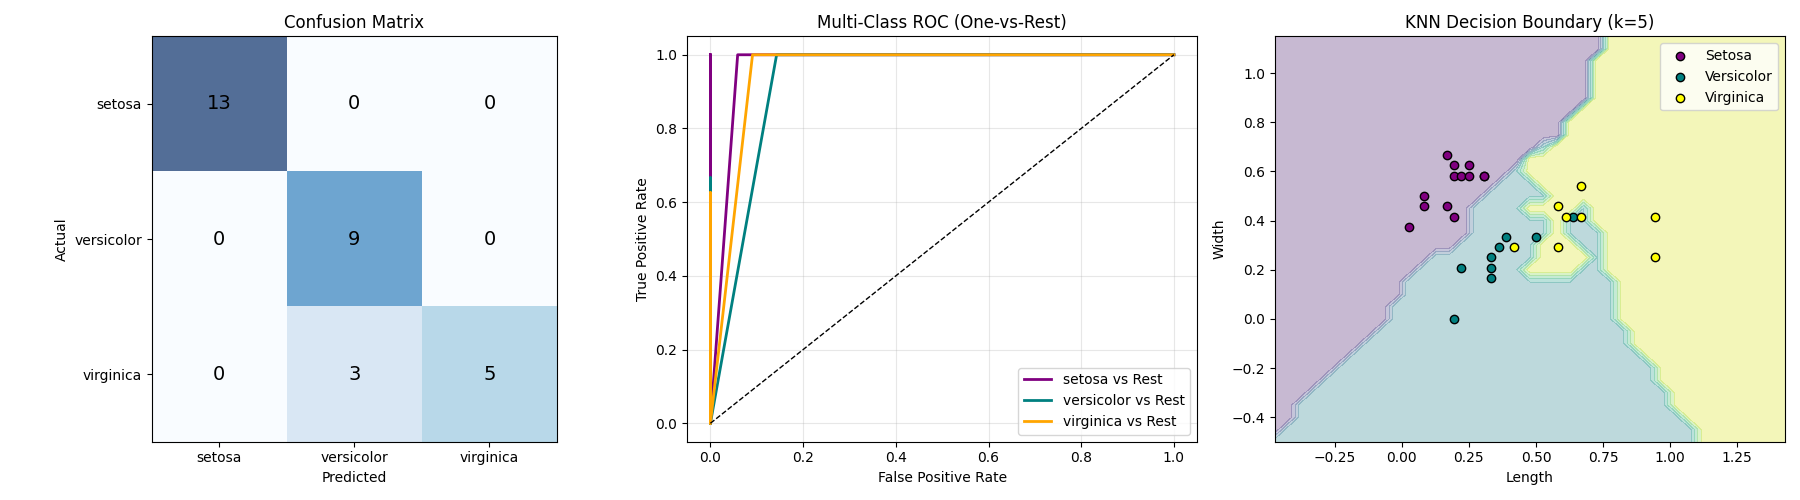
\includegraphics[width=1.0\textwidth]{knn_euclidean_results.png}
    \caption{Performance Visualization (Euclidean Metric). Left: Confusion Matrix. Middle: Multi-Class ROC Curves (One-vs-Rest). Right: Decision Boundary visualization illustrating KNN's non-linear classification.}
    \label{fig:knn_euclidean_metrics}
\end{figure}

\begin{figure}[H]
    \centering
    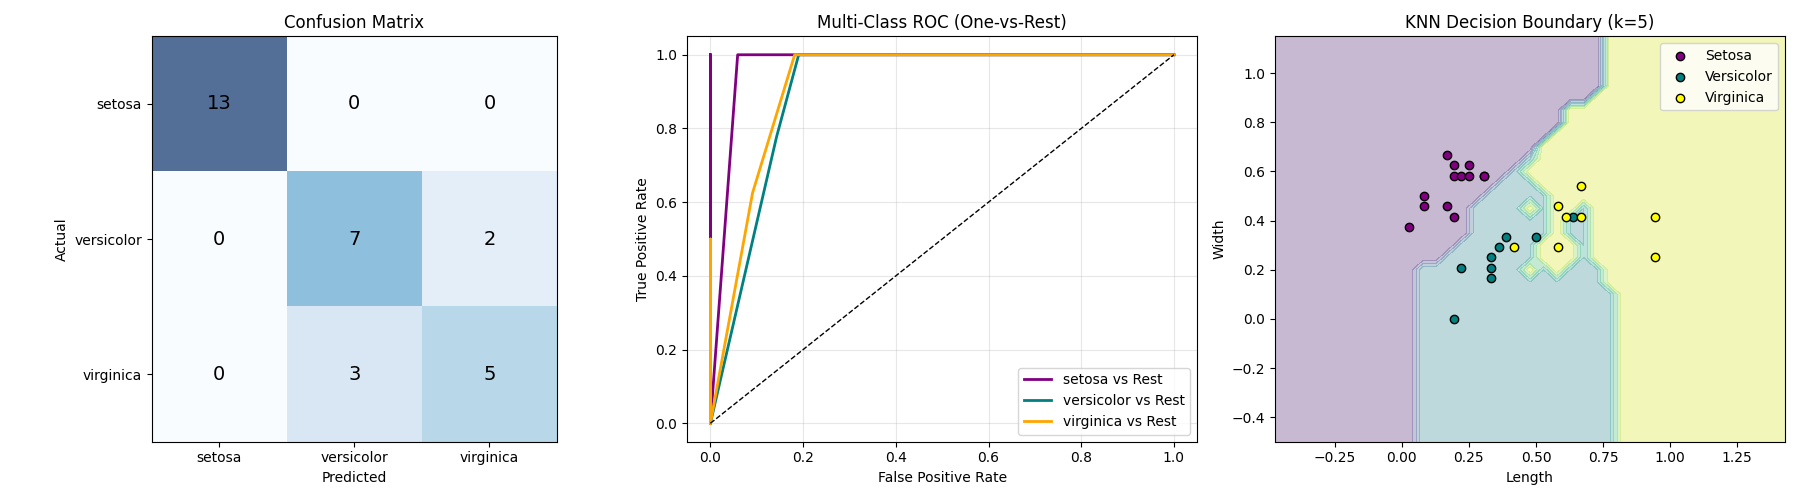
\includegraphics[width=1.0\textwidth]{knn_manhattan_results.png}
    \caption{Performance Visualization (Manhattan Metric). Left: Confusion Matrix. Middle: Multi-Class ROC Curves (One-vs-Rest). Right: Decision Boundary visualization illustrating KNN's non-linear classification.}
    \label{fig:knn_manhattan_metrics}
\end{figure}

\section{Conclusion}
The implementation of the K-Nearest Neighbors algorithm successfully classified the Iris dataset. Two distance metrics were implemented and compared: Euclidean and Manhattan. The experiment highlighted that KNN is highly effective for multi-class classification, though its performance depends heavily on the chosen distance metric. In this experiment, Euclidean distance achieved 90.00\% accuracy, outperforming Manhattan distance at 83.33\% accuracy.

The algorithm perfectly distinguishes linearly separable classes such as Setosa but encounters minor difficulties with overlapping clusters like Versicolor and Virginica. As a lazy learning algorithm, KNN incurs zero training cost but higher prediction cost ($O(N)$), making it suitable for smaller datasets where decision boundaries are irregular and non-linear.

\bibliographystyle{IEEEtran}
\renewcommand{\bibname}{References}
\addcontentsline{toc}{section}{References}
\bibliography{ref}

\end{document}
